\chapter{Implementation}
\label{chap:implementation}

\section{Front end}
Viskell is started from the \code{Main} class, which is only responsible for starting up the application. \code{Main} initializes a \code{CustomUIPane} and creates a \code{Scene} to which it is attached. The \code{CustomUIPane} class is our extension of \code{TactilePane}, a pane from the TactileFX library that adds multi-touch drag and drop behaviour to its children. We extend \code{TactilePane} with zooming and panning functionality. The class also stores references to objects used throughout the entire application, such as the \code{ConnectionCreationManager} and the Haskell environment. \code{CustomUIPane} is also responsible for application-wide gestures, like right-clicking the canvas to open a \code{FunctionMenu}, which in turn provides the user with the ability to create \code{Block} instances.

\subsection{Block structure}
As explained in the front end architecture, the visual structure of the different \code{Block} subclasses structure is expressed in \gls{FXML}. The general structure of a block consists of a top level \code{BorderPane}. The top and bottom parts are used to attach the connection anchors that the block requires, which are explicitly positioned.

Inside the center of the top level \code{BorderPane} is the block's content. For simple input- and output blocks, this is often a single element (for example a Label) representing either the input or the output. Function blocks make use of a custom \code{Pane} subclass, the \code{ArgumentSpace}, to represent its inner parts. This argument space in turn contains several input arguments, each consisting of one1 knot and one output label. The knot is used to control the knot index of the function (how many inputs are applied). The output label contains the current output type, and the \code{OutputAnchor} is always positioned in the output space (the bottom part of the top level \code{BorderPane}). Elements inside a function block are positioned from left to right.

Since the information in the labels updates often (with new type information), their length changes often as well. This results in the \code{Blocks} having to resize often. To do this, we have made extensive use of JavaFX properties. These properties let a single change somewhere in the block (like a label's size) propagate to other widths and sizes. The extensive use of properties resulted in a lot of positional aspects being defined in Java instead of FXML.

\subsection{Anchors}
Connection anchors are used to represent the input and output points of a block. Both \code{InputAnchor} and \code{OutputAnchor} extend the \code{ConnectionAnchor} class. \code{ConnectionAnchor} keeps a list of \code{Connection}s connected with it. One connection is designated the \emph{primary connection}. A \code{ConnectionAnchor} has convenience methods to get the expression of the block it's connected to, as well as a string representation of its type. Connection anchors keep track of an error state using a \code{BooleanProperty}, to which other components can listen and react when necessary. Connection anchors are a bit larger than they appear: to facilitate those with larger fingers, an extra invisible rectangle is attached below the visible anchor.

Connection anchors are given an \code{AnchorHandler} that handles the events related to creating new connections. The primary difference between input- and output anchors is that input anchors can only have one connection, while output anchors can have multiple. The anchor handler supports multi-touch events (pressed, moved and released) as well as their mouse equivalents.

\subsection{Connections}
Connections are used to connect two connection anchors. They always connect one input anchor to one output anchor. Connections are visually represented as a cubic curve, which is implemented as a subclass of \code{CubicCurve} from JavaFX. It automatically sets the bezier points, resulting in a pretty curve instead of a straight line. A connection also keeps track of its error state using a \code{BooleanProperty}, similar to how a connection anchor tracks its error state. Errors are visualized by adding an 'error' style class, which turns the connection a bright red. When adding or removing anchors from a connection, changes to connectivity will trigger an invalidation, causing the program to be reevaluated. The \code{Connection} class has lots of similar methods to supports it use in both the \code{InputAnchor} and \code{OutputAnchor} classes.

Since supporting multi-touch means that a (or multiple) user can perform multiple actions concurrently, a \code{ConnectionCreationManager} is used to link inputs to actions. Touch events already have an identifier, provided by JavaFX, but since mouse events do not have this, a fixed identification number is assigned to mouse events. Using this identification number, inputs are mapped to an action that is in progress. \code{ConnectionCreationManager} then provides several methods that perform parts of what can be considered a full action. An example of an action's part would be to instantiate a new connection with a single connection anchor. (Creating a connection from an input anchor to an output anchor is considered a full action.)

\subsection{Invalidation}
The end goal of the UI is to visually represent a program that can be shipped to the back end. In order to correctly and efficiently push chunks of the program to the back end and process the results of these chunks, an invalidation scheme is implemented. The invalidation process uses two integer values to represent the state a \code{Block} is in, namely the connection state and the visual state. These state values are used to prevent duplication of effort when traversing the graph of \code{Blocks} that make up the user's program.

The first phase of invalidation is entered upon a change in the connection state value, which is usually caused by either connecting or disconnecting a connection somewhere in the program (Figure \ref{fig:invalidation}:0). This will change the connection state property of the blocks involved, which will turn trigger a cascading reaction (Figure \ref{fig:invalidation}:1). A block first has a chance to react on the state change, and then tells all the block that are dependent on its result value of the change, by setting their connection state to the new value. When the state change can no longer be cascaded further, the next phase is entered.

After the connection state change reaches its end, the entire expression tree gets analysed. If everything goes well, this results in types being inferred for all the expressions in each of the blocks. When it does not go well, that is, if a type mismatch has occurred, the faulty input gets looked up using information from the exception a mapping of expressions to function blocks (Figure \ref{fig:invalidation}:2). The input responsible for the error has its error state set, and execution of the program is halted. Since this way only one error can be detected at a time, previous errors are remembered whenever possible to give as much information as possible. When the expression is analysed, either correctly or incorrectly, the next phase is entered.

After having found the end of the expression and having inferred the types, it is time to update the visual representation. Similar to the way the connection state cascaded, a visual state is propagated in reverse direction (Figure \ref{fig:invalidation}:2). Each \code{Block} then also reacts whenever this visual update happens, updating its labels. When the visual state can propagate no further, the invalidation is done.

Using this system it is assured that all the \code{Blocks} are fully updated before updating their visually representation and expressions are only updated and analysed when needed, separate trees won't trigger recalculation for each other.

\begin{figure}[h]
	\centering
	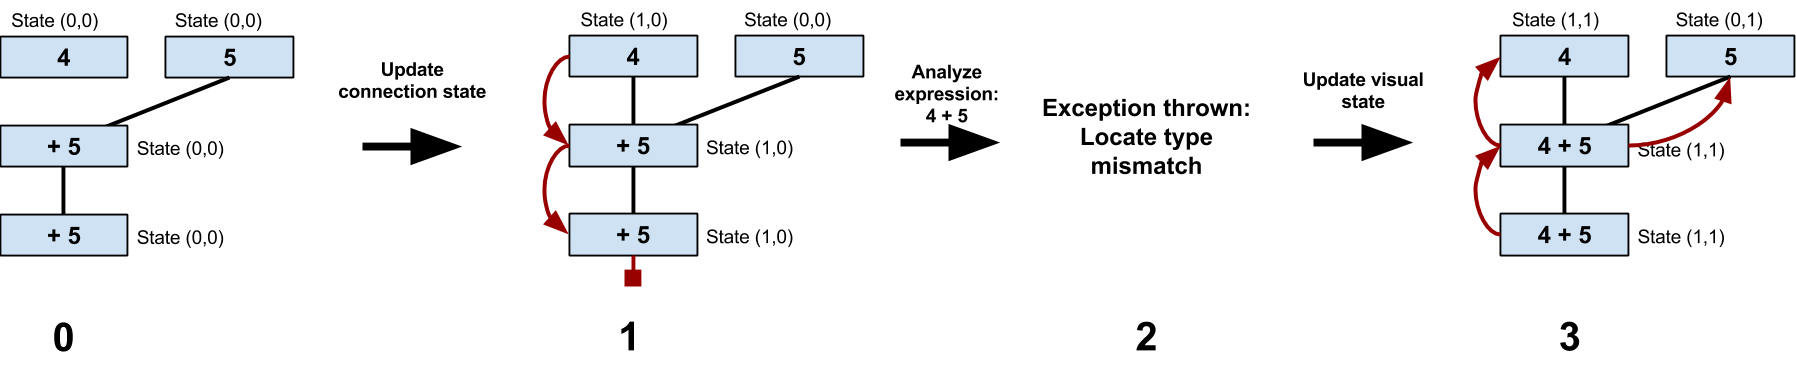
\includegraphics[width=\textwidth]{Images/invalidation}
	\caption{Invalidation scheme}
	\label{fig:invalidation}
\end{figure}

\subsection{ContextMenu}

In order to enable context specific actions in a touch environment we needed some kind of specific menu.
The CircleMenu class, an extension of the CirclePopupMenu of the JFXtras library, fulfills this role by showing a series of icons that trigger context specific actions such as copy, paste, save and delete.
As of this writing delete is the only context specific action that has been implemented.

\subsection{FunctionMenu}

The front end uses the FunctionMenu class as a main toolbar for interaction.
The menu can be called using a right click on the workspace and is constructed using a series of ListViews inside an Accordion.
Additional components have been listed inside of the Accordion as Buttons for quick and convenient access.
Each List inside of the Accordion corresponds to a catalog category in Haskell, this is done in order to make it easier for a user
to find a specific function.

\section{Back end}

\subsection{GHC integration}

The front end enables the user to construct Haskell expressions in a convenient manner.
The visual representation is converted into a tree of expression (\code{Expr}) objects and passed to the back end. \index{Expr}
The back end, finally, integrates with the Glasgow Haskell Compiler (\gls{GHC}) to do the actual computation.

The GHC integration is very simplistic.
The back end launches an instance of GHCi, the interactive read-eval-print-loop. \index{REPL}
This \gls{REPL} is then drip-fed the expressions over its standard input stream, converted from the intermediate representation into actual Haskell program code.
If the expression compiles and executes without problems, the result is returned to the front end.

\subsection{Expression and type representation}

\begin{figure}[h]
	\centering
	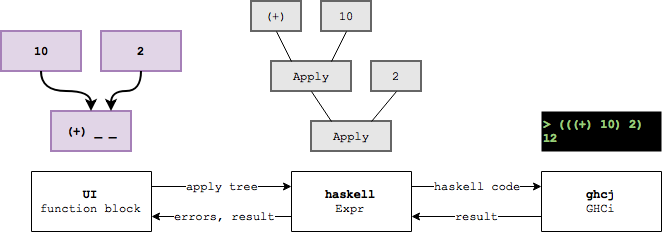
\includegraphics[scale=0.5]{Images/exprtohaskell}
	\caption{Translation from visual representation to Haskell code}
	\label{fig:exprtohaskell}
\end{figure}

\subsubsection{Expressions}
\index{function} \index{Haskell code}

To be able to work with Haskell code in Java, we built our own representation for the Haskell programming language.
We have chosen to use distinct classes (with a common superclass) for expressions that behave in a similar manner.
This object-based approach is favoured over any text based approach (including using Haskell code itself) because objects are very easy to work with.

Every expression is represented as an instance of \code{Expr} (or any subclass of \code{Expr}). \index{Expr}
An \code{Expr} is responsible for outputting syntactically correct Haskell code. \code{Expr} objects are the bridge between the tree-like graphical representation of the user interface and the textual Haskell code.
The implemented types of expressions are standard functions, values and function applications.
Each of these types of expressions share the fact that they all have a type which can be used by the type checker.

Standard functions (functions that are known to the Haskell environment) are represented as an \code{Ident} instance. \index{Ident}
This class is very simple and does not include more than the name of the function (so it can be called) and a way to lookup the type.

Values are represented in a similar way, a \code{Value} object keeps track of the string representation of the value and its type. \index{Value}
The string representation of the value should be written in a way that GHCi natively understands what is meant by it, although this is not validated.

Function application is done by using an \code{Apply} object. \index{Apply}
This class holds two expressions where the second expression is applied to the first expression.
\code{Apply} is limited to the application for a single argument.
A function with more than one argument is seen as a function with one argument that produces another function.
This way \code{Apply} allows for creating a tree like structure of a Haskell program.

Custom functions can be built using a composition of standard functions.
A custom function is defined using a \code{Function} object.
This object requires a specification of the function arguments and the expression tree of the function.
A \code{FunctionArgument} object can be used in this expression tree to use the inputs.
Functions that are defined this way will make sure that type calculations are done on a per-usage basis so reusing a function is always possible.
When a function is pushed to GHCi an \code{Ident} object is given which can be used instead of the \code{Function} object.
This comes with a great performance gain because the function itself is not continuously type checked.

Once a program has been represented as a tree of \code{Expr} objects, calling the \code{Expr.analyze()} method will invoke the type checker.
The type checker calculates the new types for the expressions in the tree.
The new types of each expression can be obtained by calling the \code{Expr.getType()} method.
This way it is possible to always get the up-to-date type of an \code{Expr} object by simply keeping a reference to it.

\begin{figure}[h]
\centering
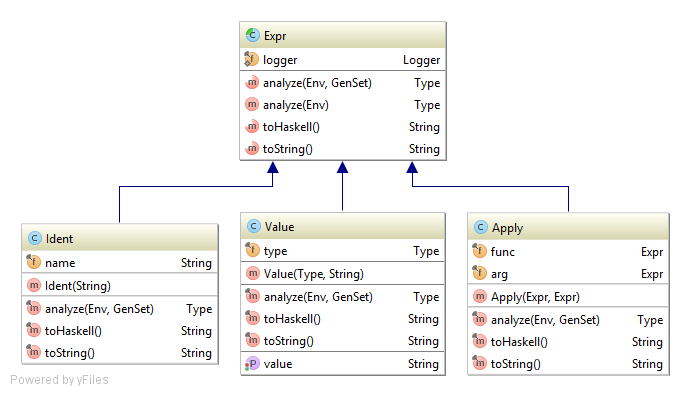
\includegraphics[scale=0.4]{Images/classdiagram-expr}
\caption{Class diagram of the Haskell expressions classes}
\label{fig:classdiagram-expr}
\end{figure}

\subsubsection{Types}
\index{type}

Types are represented similarly to expressions.
Each type is represented as an instance of \code{Type} (or any subclass of it).
The subclasses of \code{Type} are used to make working with types easier.
There is no subclass for every distinct type in Haskell, only for groups of types that are alike.

First of all types are separated into two groups: variable types and non-variable types.
Variable types are types of which the actual type is not known - types that can unify into any non-variable type (possibly with constraints).
Variable types are represented as \code{VarT}.

Non-variable types (constant types) are represented as \code{ConstT} and consist of a type constructor and a number of (optional) argument types.
A type is considered constant when it is clear which type constructor to use. A type with a known type constructor but variable types as argument types is still a constant type.

Composite types, e.g. list and tuple, are represented by respectively \code{ListT} and \code{TupleT} which are subclasses of \code{ConstT}.
These subclasses handle some validation and Haskell/string representation that is specific to these types.

Distinct Haskell types are represented as class instances, not as the class itself. The different \code{Type} subclasses make it easier to work with the types, and some are necessary in case of compound types like \code{ListT} and \code{TupleT} which are special cases.

Non-variable types can be easily compared. Two instances of the same type are equal (that is, two instances with the same base class and constructor arguments).
Variable types are only equal if it is the same instance. This is used to avoid confusion between variable types with the same name.

Type classes are represented as \code{TypeClass} instances and can be used as constraints on variable types.
Each \code{TypeClass} instance keeps a set of constant types that belong to the type class.
This information is used by the type checker to check whether a variable type is unifiable with a constant type or another variable type.

\begin{figure}[h]
\centering
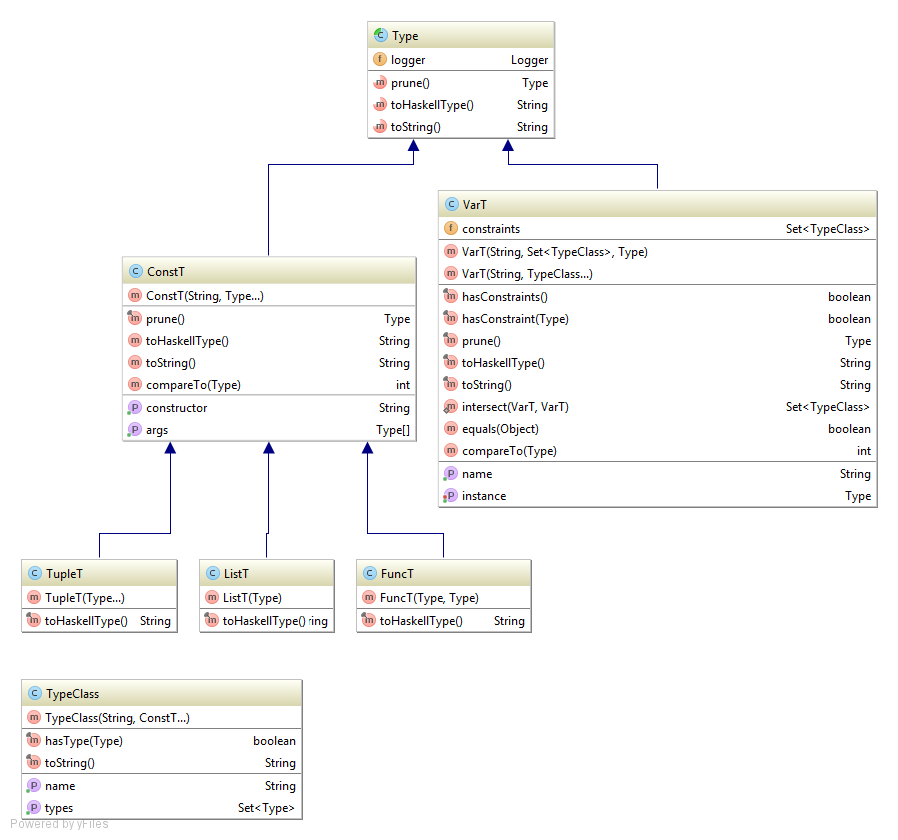
\includegraphics[scale=0.4]{Images/classdiagram-type}
\caption{Class diagram of the Haskell types classes}
\label{fig:classdiagram-type}
\end{figure}

\subsection{Type checker}
\index{type checker}

From our own experience as beginning Haskell programmers, we often encountered type errors, and therefore GHC's type error messages.
Very early in the project, we decided that the back end had to do at least some type-related work itself, to provide better errors to the user, and also to be able to show type hints, without having to parse GHC's error messages.
Not long thereafter, it was decided that such a home-grown type checker would not need to support the entirety of Haskell's type system.

After some iterations, we have arrived at an approach that could probably be described as a subset of Hindley-Milner type inference. \index{Hindley-Milner} \index{type inference}

Our (Java) implementation of Hindley-Milner type inference is based on an implementation in Scala by Andrew Forrest\cite{forrest}.
This implementation was in turn based on an implementation in Perl by Nikita Borisov\cite{borisov}.
The Perl implementation was heavily inspired by a Modula-2 implementation from 1987 by Luca Cardelli\cite{cardelli}.
Some ideas were also taken from the chapter on types from the programming languages book by Krishnamurthi\cite{plai}.

As mentioned, the type checker is not nearly powerful enough to understand or even represent the entire complexity of Haskell's type system.
However, we have found it to be `good enough' for our purposes.

\subsection{Environment management}
\index{catalog}
\index{environment}

In Haskell a lot of things depend on the environment, for example the functions that are available, the types in type classes, etc.
Our implementation solves this by introducing an environment (\code{Env}).
Objects of this class keep the types of the available functions and the type classes for every type.
Furthermore, we provide a XML-based catalog where the initial functions and type classes can be configured.
This catalog contains information that can be used by the front end, such as documentation as well.
